% Aufwandschätzung, Zeitplan, Projektplan

\section{Projektmanagement}
\label{Projektmanagement}

\subsection{Vorgehen}
\label{Projektmanagement:Vorgehen}

Für die Bachelorarbeit wurde das agile Vorgehen SCRUM in Kombination mit Elementen von \ac{RUP} gewählt.
Gründe für diese Entscheidung sind, dass das agile Vorgehen der noch zu Beginn offenen Spezifikation der \acs{ÖV}-Güteklassen und der theoretischen Aufarbeitung entgegenkommt, welche dann iterativ finalisiert werden kann und dass der theoretische Fokus der Arbeit so besser gehandhabt und schneller reagiert werden kann.
Die wöchentlichen Besprechungen und Reviews mit dem Betreuer ist ein weiterer Grund für diese Entscheidung.
Die Kombination mit Elementen von \ac{RUP} ermöglicht es, dass Projekt in einzelne Phasen aufzuteilen, um so das Ziel und die Zeit nicht aus den Augen zu verlieren und den theoretischen Teil und die Spezifikation zu einem Abschluss bringen zu können.

\subsubsection{Entwicklung}
\label{Vorgehen:Entwicklung}

Der Source-Code der Implementation wie auch diese Arbeit wird mit Git verwaltet und ist auf Github~\cite{github} abgelegt.
Die Entwicklung und das Dokumentieren erfolgt nach dem Github-Flow.
Der Master-Branch ist auf allen Repositories während der ganzen Zeit gesperrt, so dass er nur über Pull-Requests bearbeitet werden kann.
Für jedes Arbeitspaket wird ein Branch erstellt.
Ist das Arbeitspaket implementiert, wird ein Pull-Request erstellt und dem anderen Projekt-Mitglied zum Review übergeben.
Wird der Pull-Request akzeptiert, wird der Feature-Branch in den Master gemerged.
Dieses Vorgehen hat den Vorteil, dass alle Änderungen, welche in den Master gelangen, ein Review durchlaufen müssen und so die Qualität hochgehalten werden kann.


\subsection{Zeitplanung}
\label{Projektmanagement:Zeitplanung}

Die Arbeitspakte und Zeit wird mithilfe von Jira verwaltet.
Für alle Tätigkeiten werden Arbeitspakete im Backlog erfasst, priorisiert und geschätzt.
Die Schätzung der Arbeitspakete erfolgte mit Story Points.
Die Arbeitszeitverbuchung wurde auf Arbeitspaket-Stufe mit Stunden gemacht.

\subsubsection{Phasen / Iterationen und Meilensteine}
\label{Zeitplanung:Phasen / Iterationen und Meilensteine}

Die Bachelorarbeit wird in die \ac{RUP}-Phasen (Inception, Elaboration, Construction, Transition) aufgeteilt.
Dabei wird jedoch eine von der gängigen Norm abweichende Aufteilung gewählt.
Durch den theoretischen Fokus der Arbeit und der zu erarbeitenden Spezifikation wird der Elaboration das grösste Zeitbudget zugeordnet.
Dies ist auch der Grund, warum mit einwöchigen Sprints gearbeitet wird.
In den letzten zwei Wochen des Projekts wird der Aufwand pro Sprint verdoppelt (40h pro Person), da in dieser Zeit Vollzeit am Projekt gearbeitet werden kann.
Die in Tabelle \ref{table:Phasen / Iterationen und Meilensteine} definierten Meilensteine werden in Jira als Epics definiert und die Arbeitspakete diesen zugewiesen.
Dies aus dem einfachen Grund, da Jira das Konzept Milestones nicht einfach unterstützt.

\begin{landscape}
\begin{longtable}{l p{6.5cm} p{6.5cm} p{6.5cm}}
        \toprule
        \textbf{Sprint}
                                & \textbf{Sprint 1}
                                & \textbf{Sprint 2}
                                & \textbf{Sprint 3} \\

        \midrule
        \textbf{Phase}
                                & Inception
                                & Elaboration
                                & Elaboration \\

        \textbf{Milestones}
                                & \textit{Projektantrag genehmigt}
                                & \textit{Projektplan erstellt, Scope abgesteckt}
                                & \textit{Stand der Technik evaluiert}  \\

        \textbf{Inhalt}
                                & \begin{enumerate}[noitemsep]
                                    \item Projektantrag erstellen
                                    \item Grobplanung erstellen
                                    \item LaTex und CI aufsetzen
                                \end{enumerate}
                                & \begin{enumerate}[noitemsep]
                                    \item Projektplan erstellen
                                    \item FA/NFA erarbeiten
                                    \item Abgrenzungen definieren
                                \end{enumerate}
                                & \begin{enumerate}[noitemsep]
                                    \item in Norm 640 290 einarbeiten
                                    \item aktuelle Berechnungsmethodik aufschlüsseln
                                    \item Fremdsysteme \& Datenquellen eruieren
                                \end{enumerate}\\

        \toprule
        \textbf{Sprint}
                                & \textbf{Sprint 4}
                                & \textbf{Sprint 5}
                                & \textbf{Sprint 6} \\
        \midrule
        \textbf{Phase}
                                & Elaboration
                                & Elaboration
                                & Elaboration \\

        \textbf{Milestones}
                                & \textit{Stand der Technik evaluiert}
                                & \textit{technische Machbarkeit geprüft}
                                & \textit{Spezifikation umsetzungsbereit}  \\

        \textbf{Inhalt}
                                & \begin{enumerate}[noitemsep]
                                    \item Anbindung Fremdsysteme \& Datenquellen evaluieren
                                    \item Framework für Frontend evaluieren
                                    \item Auslieferung Kartendaten an Frontend evaluieren
                                \end{enumerate}
                                & \begin{enumerate}[noitemsep]
                                    \item in PostGIS einarbeiten
                                    \item Machbarkeitsanalyse pgRouting durchführen
                                \end{enumerate}
                                & \begin{enumerate}[noitemsep]
                                    \item Verbesserungen der Berechnungsmethoden erarbeiten
                                    \item Spezifikation erstellen
                                \end{enumerate}  \\

        \pagebreak
        \toprule
        \textbf{Sprint}
                                & \textbf{Sprint 7}
                                & \textbf{Sprint 8}
                                & \textbf{Sprint 9} \\

        \midrule
        \textbf{Phase}
                                & Elaboration
                                & Elaboration
                                & Construction \\

        \textbf{Milestones}
                                & \textit{Spezifikation umsetzungsbereit}
                                & \textit{End of Elaboration}
                                & \textit{Spezifikation implementiert}  \\

        \textbf{Inhalt}
                                & \begin{enumerate}[noitemsep]
                                    \item Verbesserungen der Berechnungsmethoden erarbeiten
                                    \item Spezifikation erstellen
                                \end{enumerate}
                                & \begin{enumerate}[noitemsep]
                                    \item Architektur definieren
                                    \item Infrastruktur aufsetzen
                                    \item Frontend Design Entwurf erstellen
                                \end{enumerate}
                                & \begin{enumerate}[noitemsep]
                                    \item Konfigurationsmöglichkeiten definieren
                                    \item Spezifikation umsetzen
                                \end{enumerate} \\

        \toprule
        \textbf{Sprint}
                                & \textbf{Sprint 10}
                                & \textbf{Sprint 11}
                                & \textbf{Sprint 12} \\

        \midrule
        \textbf{Phase}
                                & Construction
                                & Construction
                                & Construction \\

        \textbf{Milestones}
                                & \textit{Spezifikation implementiert}
                                & \textit{Spezifikation implementiert}
                                & \textit{Spezifikation implementiert}  \\

        \textbf{Inhalt}
                                & \begin{enumerate}[noitemsep]
                                    \item Spezifikation umsetzen
                                \end{enumerate}
                                & \begin{enumerate}[noitemsep]
                                    \item Spezifikation umsetzen
                                \end{enumerate}
                                & \begin{enumerate}[noitemsep]
                                    \item Berechnung automatisieren
                                \end{enumerate} \\

        \pagebreak
        \toprule
        \textbf{Sprint}
                                & \textbf{Sprint 13}
                                & \textbf{Sprint 14}
                                & \textbf{Sprint 15}\\

        \midrule
        \textbf{Phase}
                                & Construction
                                & Construction
                                & Construction\\

        \textbf{Milestones}
                                & \textit{Web-Applikation entwickelt}
                                & \textit{Web-Applikation entwickelt}
                                & \textit{Web-Applikation entwickelt}\\

        \textbf{Inhalt}
                                & \begin{enumerate}[noitemsep]
                                    \item Backend für Auslieferung der Kartendaten erstellen
                                    \item Frontend-Entwurf umsetzen
                                \end{enumerate}
                                & \begin{enumerate}[noitemsep]
                                    \item Backend für Auslieferung der Kartendaten erstellen
                                \end{enumerate}
                                & \begin{enumerate}[noitemsep]
                                    \item Frontend fertig stellen
                                \end{enumerate}\\

        \toprule
        \textbf{Sprint}
                                & \textbf{Sprint 16}
                                & \\
                                & \\

        \midrule
        \textbf{Phase}
                                & Transition
                                & \\
                                & \\

        \textbf{Milestones}
                                & \textit{BA abgegeben}
                                & \\
                                &  \\

        \textbf{Inhalt}
                                & \begin{enumerate}[noitemsep]
                                    \item Präsentation erstellen
                                    \item Plakat erstellen
                                    \item Arbeit finalisieren
                                    \item Arbeit abgeben

                                \end{enumerate}
                                & \\
                                & \\
        \bottomrule
    \caption{Phasen / Iterationen und Meilensteine}
    \label{table:Phasen / Iterationen und Meilensteine}
\end{longtable}
\end{landscape}

\paragraph{Fazit Projektverlauf}~\\
Im Anschluss an das Projekt lohnt es sich einen kurzen Blick auf die Abweichungen zwischen dem Geplanten und der Realität zu werfen.
Bis und mit Sprint 8 ist das Projekt mit einigen wenigen Arbeitspaketsverschiebungen analog zum Projektplan verlaufen.
Ab Sprint 9 und mit der eigentlichen Implementierung wurde uns relativ schnell bewusst, dass sich die Entwicklung der einzelnen Komponenten parallel durchführen lässt.
Der Hauptfokus und somit auch der grösste Aufwand lag jedoch immer noch bewusst auf dem \acs{ÖV}-Güteklassen 2018-Generator, da das Projekt mit diesem steht und fällt.
Nebenbei konnte jedoch Zeit in den Aufbau des Web-App und des Backend gesteckt werden.
Auch einen Frontend-Entwurf stand relativ rasch, um so keine Überraschungen gegen Ende des Projekts zu erleben.

Im Nachhinein würden wir dieses Vorgehen wieder einschlagen.
Dies aus dem Grund, dass der Generator der Kern des Projekts ist und man dadurch bei Problemen und somit Verzögerungen Abstriche bei der Web-App und Backend machen.

\subsection{Stakeholder}
\label{Projektmanagement:Stakeholder}

Im folgenden werden die Stakeholder identifiziert, genauer analysiert und in Anspruchsgruppen eingeteilt.
In Abbildung \ref{fig:stakeholder_map} ist ersichtlich, in welchem Mass diese Interesse an einem erfolgreichen Projektabschluss haben und Einfluss auf die Gestaltung des Projektes nehmen können. 
Das Interesse und der jeweilige Einfluss ist detailliert in Tabelle \ref{table:Stakeholder} aufgeführt.

Durch die Identifizierung und Gruppierung kann ein unterschiedliches Stakeholder Management durchgeführt werden. 
Die \emph{Key Player}, welche sich im oberen rechten Quadrant befinden, werden bei den Entscheidungen einbezogen, regelmässig auf den neusten Stand gebracht und aktiv ins Projekt einbezogen.
Die weniger relevanten Stakeholder im Bezug auf den Einfluss werden für das Projekt motiviert und das Interesse auf das Projektergebnis wird geweckt.

\begin{figure}[ht]
\centering
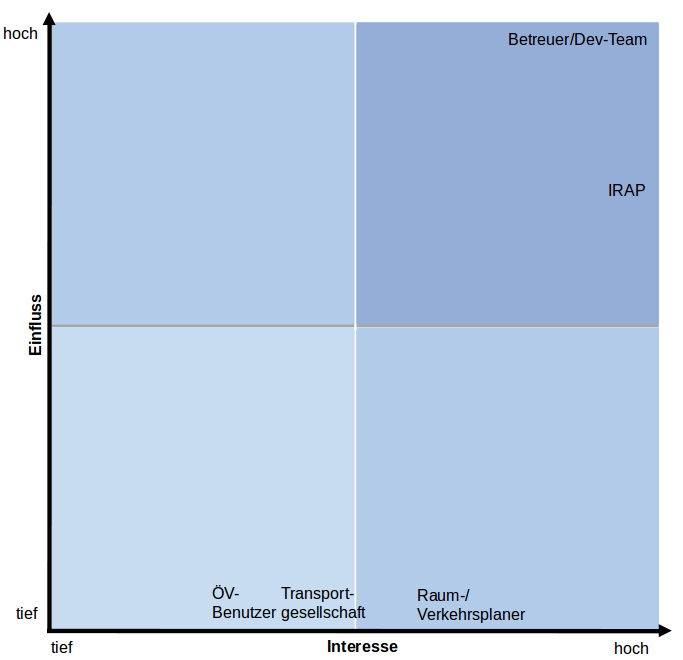
\includegraphics[width=0.7\linewidth]{projectdoc/img/stakeholder_map}
\caption[Stakeholder Map]{Stakeholder Map}
\label{fig:stakeholder_map}
\end{figure}



\begin{landscape}
\begin{longtable}{l p{9cm} p{9cm}}
        \toprule
        \textbf{Stakeholder}
                                & \textbf{Interesse}
                                & \textbf{Einfluss} \\
        \midrule
        \textbf{Betreuer (Prof. Stefan Keller)}
                                & Erfolgreiche Bachelorarbeit, welche Themengebiete des Geometa Lab tangiert und nach Abschluss einen konkreten Nutzen erbringt.
                                & Einfluss auf die Definition der Aufgabenstellung, Anforderungen, Rahmenbedingungen, laufende Steuerung des Projekts in enger Zusammenarbeit mit dem Dev-Team. \\
        \textbf{Dev-Team}
                                & Erfolgreiche Bachelorarbeit, in welcher das erlernte Wissen des Studiums konkret angewendet werden kann und das Thema „Netzwerkanalyse“ im OSM-Umfeld aufgreift. Die BA soll ein Produkt hervorbringen, welches von unterschiedlichen Personengruppen eingesetzt werden kann.
                                & Einfluss auf die Definition der Aufgabenstellung, Anforderungen,  Rahmenbedingungen, laufende Steuerung des Projekts in enger Zusammenarbeit mit dem Betreuer. \\                                
        \textbf{IRAP (Prof. Claudio Büchel)}
                                & Interessen analog zu Raumplaner/Verkehrsplaner. Durch die praktische Erfahrung mit der bisherigen Norm existiert ein aktives Interesse, diese neu zu gestalten und für die Zukunft fit zu machen.
                                & Nimmt die \gls{OeVGK18}-Spezifikation ab und gestaltet die Spezifikation aktiv mit. \\
        \textbf{Raumplaner/Verkehrsplaner}
                                & Gemäss Verordnung werden nur noch Gebiete mit einer guten ÖV-Erschliessung verdichtet. Mit den Güteklassen lässt sich prüfen, an welchen Standorten eine Verdichtung stattfinden kann.
                                & Hat keinen direkten Einfluss. Die Interessen fliessen in die Anforderungen. \\     
        \textbf{Transportgesellschaften}
                                & Transportgesellschaften überprüfen mit den Güteklassen die aktuelle Erschliessung der Schweiz und können dadurch Erweiterungspotential eruieren.
                                & Hat keinen direkten Einfluss. Die Interessen fliessen in die Anforderungen. \\       
        \textbf{Dev-Team}
                                & ÖV-Benutzer, welcher auf der Wohnungssuche ist, prüft mit den Güteklassen die Erschliessung eines potentiellen Wohnortes.
                                & Hat keinen direkten Einfluss. Die Interessen fliessen in die Anforderungen. \\                                                   
        \bottomrule
    \caption{Stakeholder}
    \label{table:Stakeholder}
\end{longtable}
\end{landscape}

\subsection{Risiken}
\label{Projektmanagement:Risiken}

\begin{table}[ht]
    \begin{tabular}{p{0.5cm} p{7cm} p{2cm} p{2cm} p{2cm}}
        \toprule
        \textbf{ID}
        & \textbf{Risiko}
        & \textbf{max. Schaden [h]}
        & \textbf{WSK}
        & \textbf{gewichteter Schaden} \\
        \midrule
        \textbf{1}
                        & Definition der \gls{OeVGK18}-Spezifikation findet kein Ende.
                        & 20
                        & 30\%
                        & 6 \\
        \textbf{2}
                        & PostGIS und pgRouting eignet sich nicht für die \acs{ÖV}-Güteklasse-Berechnung.
                        & 40
                        & 25\%
                        & 10 \\
        \textbf{3}
                        & PostGIS und pgRouting sind technologisches Neuland.
                        & 24
                        & 30\%
                        & 7.2 \\
        \textbf{4}
                        & Es existieren viele Abhängigkeiten auf Fremdsysteme.
                        & 8
                        & 20\%
                        & 1.6 \\
        \textbf{5}
                        & Fremdsysteme bieten nicht die geforderte Datenqualität.
                        & 24
                        & 20\%
                        & 4.8 \\
        \textbf{6}
                        & Frontend-Framework eignet sich nicht für Karten-Integration.
                        & 16
                        & 30\%
                        & 4.8 \\
        \bottomrule
    \end{tabular}
    \caption{Risiken}
    \label{table:Risiken}
\end{table}

In der Tabelle \ref{table:Risiken} sind die identifizierten Projektrisiken aufgelistet.
Grundsätzlich lässt sich sagen, dass sich alle Risiken in einem vertretbaren Rahmen befinden.
Das Hauptrisiko der Bachelorarbeit ist das technische Neuland und die fehlende Erfahrung mit PostGIS und pgRouting.
Der Umgang und die Konsequenzen, welche sich aus der Risikoanalyse ableiten, sind in den folgenden Unterkapitel beschrieben.
Die Risiken werden in einem zwei-wöchentlichen Rhythmus diskutiert und bei Unstimmigkeiten revidiert und neue Massnahmen getroffen.

\begin{figure}[ht]
    \centering
    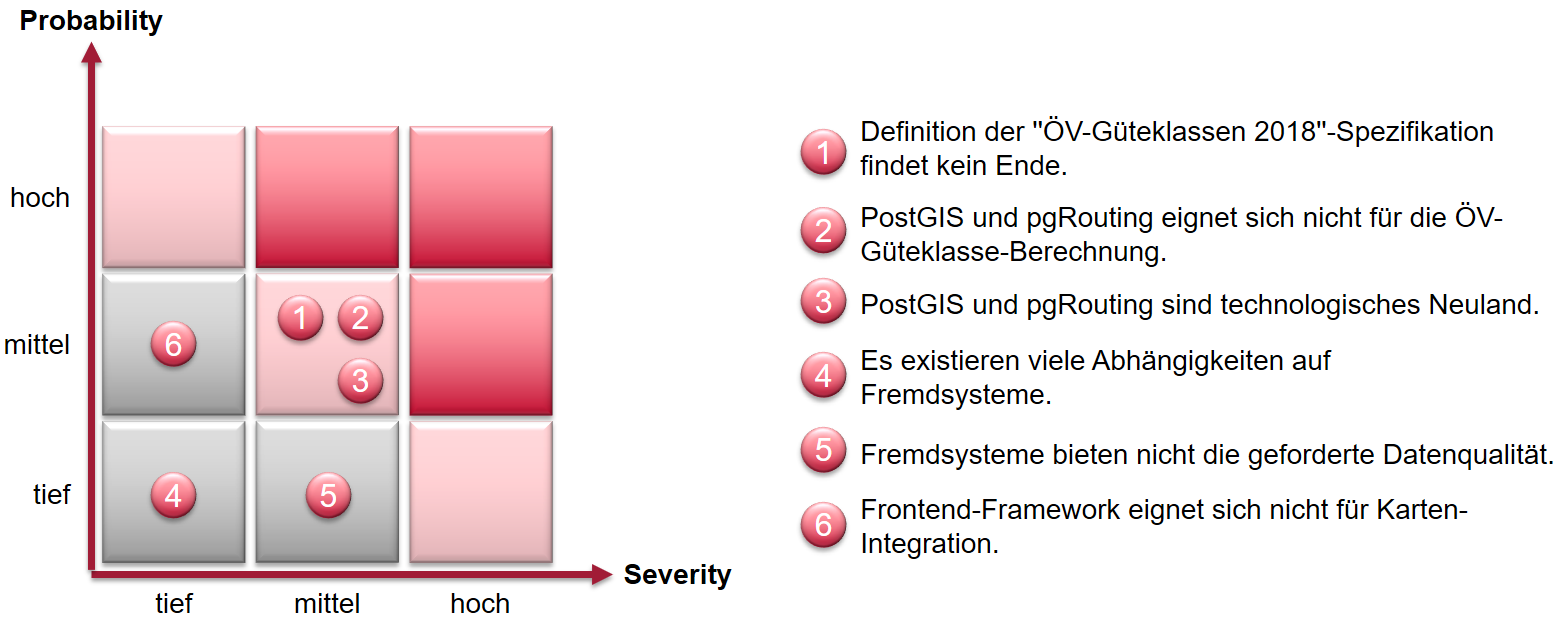
\includegraphics[width=1.0\linewidth]{projectdoc/img/risk_analysis}
    \caption[Risiko-Analyse]{Risiko-Analyse}
    \label{fig:risk_analysis}
\end{figure}

\subsubsection{Umgang mit Risiken}
\label{Risiken:Umang mit Risiken}

Die Risikoanalyse hat einen erwarteten Mehraufwand von \emph{34.4} Stunden ergeben.
Den in Tabelle \ref{table:Risiken} identifizierten technischen Risiken (\emph{ID 2, 3 und 6}) wird mit einer geplanten Einarbeitung und Prototypen entgegen gewirkt.
Damit die Spezifikation der \gls{OeVGK18} ein definitives Ende findet und mit der Umsetzung begonnen werden kann, wird ein fixer Milestone "`Spezifikation umsetzungsbereit"' definiert, welcher zwei Überarbeitungsrunden beinhaltet.

\subsubsection{Konsequenz}
\label{Risiken:Konsequenz}

Falls die geplanten Massnahmen nicht den erwarteten Nutzen zeigen oder unerwartete Stolpersteine auftreten, wird der Use Case \nameref{Use Cases:UC05} aus dem Scope gestrichen.

\subsubsection{Risiko-Refinement}
\label{Risiken:Risiko-Refinement}

Alle zwei Wochen findet ein Risiko-Refinement statt.
Zweck dieses Meeting ist es, dass die Risiken mit der aktuellen Situation abgeglichen werden.
Bei Bedarf kann so rasch auf eintretende Risiken reagiert und mit den betroffenen Stakeholder einen Konsens über das weitere Vorgehen gefunden werden.
